% This is text associated with the open textbook "Open Electromagnetics"
% See immediately below for author, date
% This work is licensed under the Creative Commons Attribution-ShareAlike 4.0 International License. (CC BY-SA 4.0) 
% To view a copy of the license, visit http://creativecommons.org/licenses/by-sa/4.0/

%ORB TITLE Faraday's Law
%ORB AUTHOR 0        # S.W. Ellingson, Virginia Tech (ellingson@vt.edu)
%ORB DATE 20180807   # yyyymmdd
%ORB ABSTRACT Faraday's Law: Single-loop equation, explains procedure to get emf, explains types of emf

\label{m0055_Faradays_Law} % <-- Must match name of this file and module directory name.  Don't mess with this!
\index{Faraday's law|(}

Faraday's Law describes the generation of electric potential by a time-varying magnetic flux.
\index{flux!magnetic}
This is a form of \emph{electromagnetic induction}, 
\index{induction}
as discussed in Section~\ref{m0129_Electromagnetic_Induction}.

To begin, consider the scenario shown in Figure~\ref{m0055_fFaradaySingleLoop}. A single loop of wire in the presence of an impressed magnetic field ${\bf B}$. 
For reasons explained later, we introduce a small gap and define $V_T$ to be the potential difference measured across the gap according to the sign convention indicated.
The resistance $R$ may be any value greater than zero, including infinity; i.e., a literal gap.
%
\begin{figure}[b!]
\begin{center}
\pdftooltip{{  % note double braces
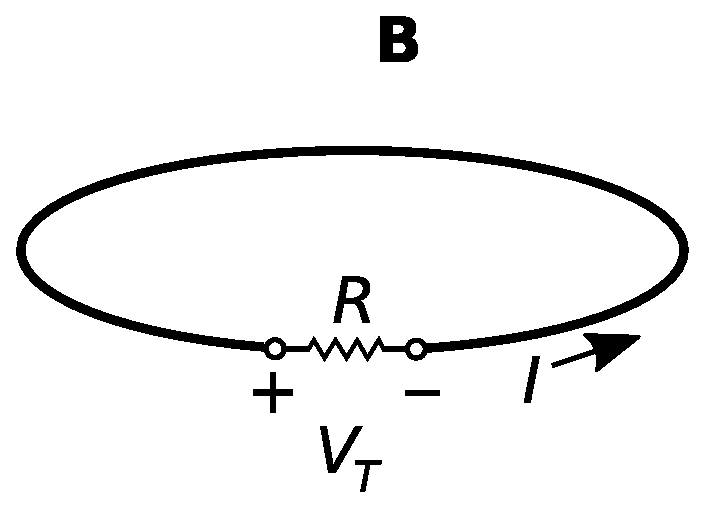
\includegraphics[width=2in]{modules/m0055_fFaradaySingleLoop.eps}
}}{A loop of wire lying in a magnetic field, B. In the loop lies a resistor, R, between a positive and negative node. Beneath the resistor is labeled V sub T. A vector, I, on the right points in a counterclockwise direction.}
\end{center} 
% ***WikipediaCommonsURL
%\centerline{\scriptsize 
%\copyright~\hyperref[***_Credit]{author} 
%\href{https://creativecommons.org/licenses/by-sa/4.0/}{CC BY-SA 4.0} 
%} 
\caption{
\label{m0055_fFaradaySingleLoop}
A single loop of wire in the presence of an impressed magnetic field.
}
\end{figure}

As long as $R$ is not infinite, we know from Lenz's Law 
\index{Lenz's law}
(Section~\ref{m0129_Electromagnetic_Induction}) to expect that a time-varying magnetic field will cause a current to flow in the wire. 
Lenz's Law also tells us the direction in which the current will flow.
However, Lenz's Law does not tell us the magnitude of the current, and it sidesteps some important physics that has profound implications for the analysis and design of electrical devices, including generators and transformers.

The more complete picture is given by Faraday's Law.
In terms of the scenario of Figure~\ref{m0055_fFaradaySingleLoop}, Faraday's Law relates the potential $V_T$ induced by the time variation of ${\bf B}$. 
$V_T$ then gives rise to the current identified in Lenz's Law. 
The magnitude of this current is simply $V_T/R$. %, oriented in the direction shown in Figure~\ref{m0055_fFaradaySingleLoop}.
Without further ado, here's Faraday's Law for this single loop scenario:
%
\begin{equation}   
V_T = - \frac{\partial}{\partial t} \Phi ~~\mbox{(single loop)}
\label{m0055_eVT}
\end{equation}
%
Here $\Phi$ is the magnetic flux (units of Wb) associated with any open surface $\mathcal{S}$ bounded by the loop:
%
\begin{equation}   
\Phi = \int_{\mathcal{S}} { {\bf B} \cdot d{\bf s} }
\label{m0055_ePhi}
\end{equation}
%
where ${\bf B}$ is magnetic flux density (units of T or Wb/m$^2$) and $d{\bf s}$ is the differential surface area vector.

To make headway with Faraday's Law, one must be clear about the meanings of $\mathcal{S}$ and $d{\bf s}$.
If the wire loop in the present scenario lies in a plane, then a good choice for $\mathcal{S}$ is the simply the planar area bounded by the loop.
However, \emph{any} surface that is bounded by the loop will work, including non-planar surfaces that extend above and/or below the plane of the loop. All that is required is that every magnetic field line that passes through the loop also passes through $\mathcal{S}$. 
This happens automatically if the curve $\mathcal{C}$ defining the edge of the open surface $\mathcal{S}$ corresponds to the loop.
Subsequently, the magnitude of $d{\bf s}$ is the differential surface element $ds$ and the direction of $d{\bf s}$ is the unit vector $\hat{\bf n}$ perpendicular to each point on $\mathcal{S}$, so $d{\bf s}=\hat{\bf n}ds$.

This leaves just one issue remaining -- the orientation of $\hat{\bf n}$.  
This is sorted out in Figure~\ref{m0055_fFaradaySingleLoopSC}.
There are two possible ways for a vector to be perpendicular to a surface, and the direction chosen for $\hat{\bf n}$ will affect the sign of $V_T$.  
Therefore, $\hat{\bf n}$ must be somehow related to the polarity chosen for $V_T$.  Let's consider this relationship.
Let $\mathcal{C}$ begin at the ``$-$'' terminal of $V_T$ and follow the entire perimeter of the loop, ending at the ``$+$'' terminal.
Then, $\hat{\bf n}$ is determined by the following ``right-hand rule:''
\index{right-hand rule!Stokes' theorem}
$\hat{\bf n}$ points in the direction of the curled fingers of the right hand when the thumb of the right hand is aligned in the direction of $\mathcal{C}$.
It's worth noting that this convention is precisely the convention used to relate $\hat{\bf n}$ and $\mathcal{C}$ in Stokes' Theorem 
\index{Stokes' theorem}
(Section~\ref{m0051_Stokes_Theorem}).
%
\begin{figure}
\begin{center}
\pdftooltip{{  % note double braces
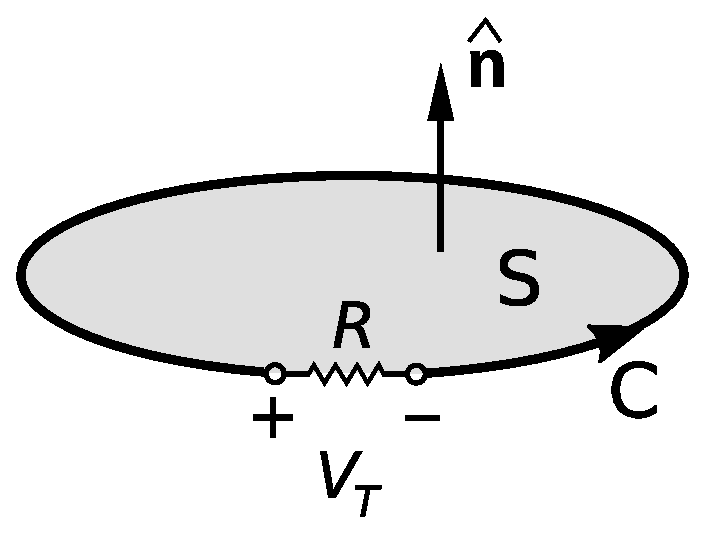
\includegraphics[width=2in]{modules/m0055_fFaradaySingleLoopSC.eps}
% ***WikipediaCommonsURL
}}{A circular surface, S, bounded by C. On C, an arrow points in a counterclockwise direction. In the loop of C lies a resistor, R, between a positive and negative node. Beneath the resistor is labeled V sub T. A vector comes out of the surface, labeled n-hat. }
\end{center} 
%\centerline{\scriptsize 
%\copyright~\hyperref[***_Credit]{author} 
%\href{https://creativecommons.org/licenses/by-sa/4.0/}{CC BY-SA 4.0} 
%} 
\caption{
\label{m0055_fFaradaySingleLoopSC}
Relationship between the polarity of $V_T$ and orientations of $\mathcal{C}$ and $\hat{\bf n}$ in the planar single-loop scenario.
}
\end{figure}

Now let us recap how Faraday's Law is applied to the single loop scenario of Figure~\ref{m0055_fFaradaySingleLoop}:
%
\begin{enumerate}
\item Assign ``$+$'' and ``$-$'' terminals to the gap voltage $V_T$.
\item The orientation of $\hat{\bf n}$ is determined by the right hand rule, taking the direction of $\mathcal{C}$ to be the perimeter of the loop beginning at ``$-$'' and ending at ``$+$''
\item ${\bf B}$ yields a magnetic flux $\Phi$ associated with the loop according to Equation~\ref{m0055_ePhi}. $\mathcal{S}$ is any open surface that intersects all the magnetic field lines that pass through the loop (so you might as well choose $\mathcal{S}$ in a way that results in the simplest possible integration).
\item By Faraday's Law (Equation~\ref{m0055_eVT}), $V_T$ is the time derivative of $\Phi$ with a change of sign.
\item The current $I$ flowing in the loop is $V_T/R$, with the reference direction (i.e., direction of positive current) being from ``$+$'' to ``$-$'' through the resistor.  Think of the loop as a voltage source, and you'll get the correct reference direction for $I$.
\end{enumerate}

At this point, let us reiterate that the electromagnetic induction described by Faraday's Law induces \emph{potential} (in this case, $V_T$) and not \emph{current}.
The current in the loop is simply the induced voltage divided by the resistance of the loop.  
This point is easily lost, especially in light of Lenz's Law, which seems to imply that current, as opposed to potential, is the thing being induced.

Wondering about the significance of the minus sign in Equation~\ref{m0055_eVT}?  That is specifically Lenz's Law:  
The current $I$ that ends up circulating in the loop generates its own magnetic field (``${\bf B}_{ind}$'' in Section~\ref{m0129_Electromagnetic_Induction}), which is distinct from the impressed magnetic field ${\bf B}$ and which tends to oppose change in ${\bf B}$.  Thus, we see that Faraday's Law subsumes Lenz's Law.   

Frequently one is interested in a structure that consists of multiple identical loops.
We have in mind here something like a coil with $N\ge1$ windings tightly packed together.
In this case, Faraday's Law is 
%
\begin{equation}   
\boxed{
V_T = - N\frac{\partial}{\partial t} \Phi
}
\label{m0055_eVTN}
\end{equation}
%
Note that the difference is simply that the gap potential $V_T$  is greater by $N$.  
In other words, each winding of the coil contributes a potential given by Equation~\ref{m0055_eVT}, and these potentials add in series.

%ORB HIGHLIGHT
\begin{mdframed}[backgroundcolor=yellow!20,nobreak=true] 
Faraday's Law, given in general by Equation~\ref{m0055_eVTN}, states that the potential induced in a coil is proportional to the time derivative of the magnetic flux through the coil.
\end{mdframed}

The induced potential $V_T$ is often referred to as ``emf,'' 
\index{electromotive force|see{emf}}
\index{emf}
\index{force!electromotive|see{emf}}
which is a contraction of the term {\it electromotive force} -- a misnomer to be sure, since no actual force is implied, only potential.
The term ``emf'' is nevertheless frequently used in the context of Faraday's Law applications for historical reasons.
 
Previously in this section, we considered the generation of emf by time variation of ${\bf B}$.
However, Equation~\ref{m0055_eVT} indicates that what actually happens is that the emf is the result of time variation of the magnetic flux, $\Phi$.
Magnetic flux is magnetic flux density integrated over area, so it appears that emf can also be generated simply by varying $\mathcal{S}$, independently of any time variation of ${\bf B}$. 
In other words, emf may be generated even when ${\bf B}$ is constant, by instead varying the shape or orientation of the coil.
So, we have a variety of schemes by which we can generate emf. 
Here they are:
%
\begin{enumerate}
\item Time-varying ${\bf B}$ (as we considered previously in this section).  For example, ${\bf B}$ might be due to a permanent magnet that is moved (e.g., translated or rotated) in the vicinity of the coil, as described in Section~\ref{m0129_Electromagnetic_Induction}.  Or, more commonly, ${\bf B}$ might be due to a different coil that bears a time-varying current.  These mechanisms are collectively referred to as {\it transformer emf}. 
\index{emf!transformer}
\index{transformer!emf|see{emf}}
Transformer emf is the underlying principle of operation of transformers; for more on this see Section~\ref{m0031_Transformers_Principle_of_Operation}.
\item The perimeter $\mathcal{C}$ -- and thus the surface $\mathcal{S}$ over which $\Phi$ is determined -- can be time-varying.  For example, a wire loop might be rotated or changed in shape in the presence of a constant magnetic field.  This mechanism is referred to as {\it motional emf}
\index{motional emf|see{emf}}
\index{emf!motional}
and is the underlying principle of operation of generators 
\index{generator}
(Section~\ref{m0030_Electric_Generator}).
\item Transformer and motional emf can exist in various combinations. From the perspective of Faraday's Law, transformer and motional emf are the same in the sense in either case $\Phi$ is time-varying, which is all that is required to generate emf.
\end{enumerate}

Finally, a comment on the generality of Faraday's Law.
Above we have introduced Faraday's Law as if it were specific to loops and coils of wire.
However, the truth of the matter is that Faraday's Law is fundamental physics.  If you can define a closed path -- current-bearing or not -- then you can compute the potential difference achieved by traversing that path using Faraday's Law.  The value you compute is the potential associated with electromagnetic induction, and exists independently and in addition to the potential difference associated with the static electric field (e.g., Section~\ref{m0064_V_due_to_Point_Charges}).   
In other words:
%
%ORB HIGHLIGHT
\begin{mdframed}[backgroundcolor=yellow!20,nobreak=true] 
Faraday's Law indicates the contribution of electromagnetic induction 
\index{induction}
(the generation of emf by a time-varying magnetic flux) to the potential difference achieved by traversing a closed path.
\end{mdframed}

In Section~\ref{m0050_Maxwell-Faraday_Equation}, this insight is used to transform the static form of Kirchoff's Voltage Law 
\index{Kirchoff's voltage law!electrostatics}
(Section~\ref{m0016_Kirchoffs_Voltage_Law_Electrostatics_Integral_Form}) -- which gives the potential difference associated with electric field only -- into the \emph{Maxwell-Faraday Equation}
\index{Maxwell-Faraday equation}
(Section~\ref{m0050_Maxwell-Faraday_Equation}), which is a general statement about the relationship between the instantaneous value of the electric field and the time derivative of the magnetic field.

%%%%%%%%%%%%%%%%%%%%%%%%%%%%%%%%%%%%%%%%%%%%%%%%%%%%%%%%%%%%

{\bf Additional Reading:}
\begin{itemize}
\item ``\href{https://en.wikipedia.org/wiki/Faraday's_law_of_induction}{Faraday's law of induction}'' on Wikipedia.
\end{itemize}

\index{Faraday's law|)}
